\section{Ejercicio 1}
\subsection{El Problema}
Dado dos cadenas de caracteres $W$ y $P$, se desea saber si $P$ es una subcadena de $W$.\\
Formalmente, se define $W = [w_1,...,w_N]$ y $P = [p_1,...,p_k]$, y se desea saber si existe $W_P = [w_q,...,w_t] = P$, con $1 \leq q \leq t \leq N$.\\
El algoritmo debe tener complejidad \O{N}.

\subsection{Desarrollo}
Para resolver el problema, se utilizó el algoritmo de \emph{Knuth-Morris-Pratt}.
Por lo tanto, la solución se divide en dos partes:
\begin{itemize}
	\item Calcular los bordes de la cadena $P$
	\item Buscar si existe $W_P$
\end{itemize}

\subsubsection{Cálculo de bordes}
Al momento de realizar la búsqueda de $W_P$, la solución más ingenua constaría de contrastar $P$ con todas las subcadenas de $W$ de tamaño $|P|$. Para lograrlo, se debería ir desplazando $P$ una posición a la vez, y ver si se corresponde con alguna subcadena de $W$, de la siguiente manera:

\begin{figure}[h]
	\centering
	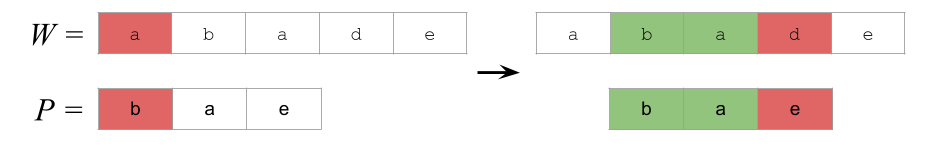
\includegraphics[width=\textwidth]{Imagenes/Ejercicio1/Shift.png}
	\caption{Ejemplo de cadena siendo desplazada de a una posición}
\end{figure}

Este método es muy ineficiente y tiene complejidad \O{|P|*|W|}.
Esto se debe a que el dicha solución realiza desplazamientos que son inválidos, es decir, desplazar $P$ en una posición es seguro que no se va a corresponder y que va a fallar, como en el siguiente ejemplo:

\begin{figure}[H]
	\centering
	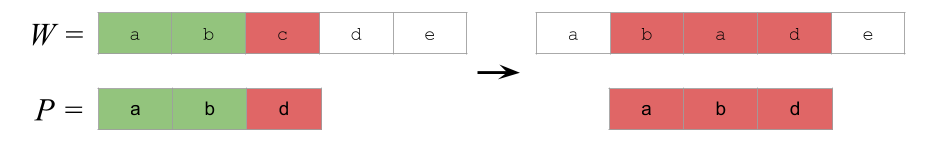
\includegraphics[width=\textwidth]{Imagenes/Ejercicio1/ShiftInvalido.png}
	\caption{Ejemplo de desplazamiento que conlleva a falla}
\end{figure}

El cálculo de los bordes de la cadena $P$ se realiza a modo de precomputo para la búsqueda de $W_P$, y previene que se realicen dichos desplazamientos inválidos. Llamaremos $\Pi$ a la estructura que guarda dicha información.
Algunas definiciones:
\begin{itemize}
	\item $P_k \sqsubset P_i \Leftrightarrow P_k$ es prefijo de $P_i$. Analogamente vale $P_k \sqsupset P_i$
	\item $\pi_i = max \{k: k < i \wedge P_k \sqsupset P_q\}$
	\item $\Pi = [\pi_1,...,\pi_{|P|}]$
\end{itemize}

En esta sección explicaremos cómo calcular $\Pi$, sin embargo su utilidad se verá en la sección siguiente.

\subsubsection{Complejidad}

\subsection{Puntaje}
El peso otorgado a este ejercicio es:
